
\section{Discussion}
\label{sec: discussion}

\autoref{thm: convergence mcopi uniform} showed that initial-visit MC-O-PI converges almost surely to $\qopt$ 

when updates are uniform over the actions in each state.








This section explores the implications of this result.
We first explain that the uniformity condition effectively requires using initial-visit updates, which does not necessarily slow down convergence compared to first-visit updates.
We then describe how to generalise this result to optimistic policy-iteration algorithms with temporal-difference updates, or when the estimate $q_k$ is stored approximately at every step.
Finally, we discuss the roles of cumulative learning, step-size regularity and policy ties.








\subsection{Uniform updates effectively force initial-visits}


When the underlying MDP is unknown, using first- or every-visit updates causes the update distribution $\mu_k$ to depend on the unknown transition dynamics induced by policy $\pi_k$.
Therefore, requiring uniform update distributions effectively forces the use of initial-visit updates,

because by updating only the initial state-action pair of each episode, we ensure $\mu_k$ equals $\sigma_k$ and thus retain control.

This control comes at the cost of data efficiency: the initial-visit method discards within-episode transitions that the first-visit method would reuse. However, more updates per episode do not automatically translate into faster policy convergence.
The extra updates induce a bias in the update distribution that can generate sliding modes in the action-value estimates $(q_k)_{k \ge 0}$ and thereby slow down the convergence of the policy sequence $(\pi_k)_{k \ge 0}$. Ultimately, it is the convergence speed of this policy sequence that truly matters for identifying the optimal behaviour of the MDP.


To illustrate this, consider the MDP in \autoref{fig: experiment smallest MDP for iv vs fv} with a discount factor $\discount = 0.5$. Action \textit{left} yields a reward of one and \textit{right} yields a reward of zero.


Under a uniform sampling distribution $\sigma_k$, the intial-visit method updates exactly one state-action pair per episode, whereas the first-visit method updates on average $1.5$ pairs.
With a learning rate $\alpha_k = 1/(k+100)$, the first-visit method also benefits from larger effective steps because it updates state-action pairs more frequently.



Despite this apparent advantage, the initial-visit method is more stable than first-visit when MC-O-PI is initialised above $\qopt$.
Namely, initial-visit solutions follow straight lines that always point towards better policies.
In contrast, first-visit solutions exhibit a sliding mode that causes high-frequency oscillations in the policy sequence and traps $q_k$ near the boundary for longer.
As a result, first-visit can take longer to settle on the optimal policy.
For instance, when averaging over 1000 solutions starting in $q'$, first-visit ones require on average 43 updates to settle on $\pi_*$, whereas initial-visit ones always remain in $\region(\best{\pi})$.
When starting in $q$, the solutions take 68 and 70 updates to settle on $\pi_*$.


Overall, this experiment illustrates that the initial-visit method can be practical in real-world applications. 
By avoiding sliding modes, it sometimes converges to the optimal policy $\best{\pi}$ as fast as, or faster than, the first-visit method despite fewer updates and smaller effective learning rates.
Besides, the initial-visit method is more reliable for early stopping. Namely, if training stops early, the last greedy policy of an initial-visit solution is typically the best policy encountered so far, whereas the first-visit solution may be oscillating across a decision boundary, making it unclear which policy is best.
















\begin{figure}[t!]
    \centering
    \begin{subfigure}[b]{\textwidth}
        \centering




















        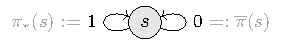
\includegraphics[width=0.35\linewidth]{figures/mdp.pdf}
        \caption{MDP}
        \label{fig: experiment smallest MDP for iv vs fv}
    \end{subfigure}%
    \\
    \vspace{0.5cm}

    \begin{subfigure}[b]{0.48\textwidth}



















                







                


                

                



                




        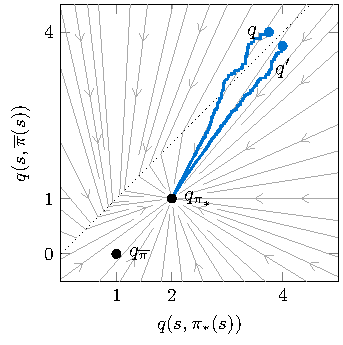
\includegraphics[width=0.8\linewidth]{figures/iv-sol.pdf}
        \caption{Initial-visit solutions}
        \label{fig: iv versus fv simulations IV}
    \end{subfigure}
    \hfill

    \begin{subfigure}[b]{0.48\textwidth}



















                







                


                

                



                




        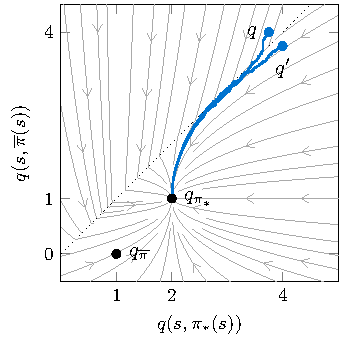
\includegraphics[width=0.8\linewidth]{figures/fv-sol.pdf}
        \caption{First-visit solutions}
        \label{fig: iv versus fv simulations FV}
    \end{subfigure}
    \caption{By avoiding sliding modes, initial-visit solutions sometimes converge to the optimal policy $\best{\pi}$ faster than first-visit solutions despite fewer updates and smaller effective learning rates. The blue lines are MC-O-PI solutions starting in $q$ or $q'$, whereas the grey lines indicate the mean-field flow.}
    \label{fig: iv versus fv simulations}
\end{figure}





















































































\subsection{Mean-field analysis with temporal difference updates}
\label{sec: discussion temporal difference}

The gap estimate uses conditional drift and variance bounds, while the favorable-update construction uses a bounded number of requests regardless of the waiting time. An analogous approach to temporal-difference updates would additionally need a policy-improvement mechanism and a favorable-update construction compatible with targets that change with the current estimate. The present theorem does not establish those properties.
The additional difficulty would be to understand how the position of the estimate $q$ and the depth $n$ of the episode simulations affect the target $T_{\pi}^n q$, where $\pi \in P(q)$ and $T_\pi$ is the Bellman operator associated with policy $\pi$.




\subsection{MC-O-PI with function approximation}
\label{sec: discussion function approximation}

\autoref{thm: convergence mcopi uniform} applies specifically to \textit{tabular} MC-O-PI, where the estimate $q_k$ can be stored exactly.
In practical applications, however, the estimate is approximated, for instance using a neural network.
In this setting, the error between the observed return and the current estimate is then used to update the parameters of the approximation.


With a sufficiently rich approximation method,
the approximation error should only contribute a finite perturbation to the MC-O-PI difference inclusion.
This suggests that \autoref{thm: convergence mcopi uniform}
can be generalised with function approximation using the results in \citep[Section~4.3.3]{Bertsekas1996Neuro-DynamicProgramming} or \citep[Section~5.2]{Kushner2003StochasticApplications}.








Finally, recent breakthroughs in natural language processing and robotics~\citep{Schulman2017ProximalAlgorithms} rely on policy gradient methods.
\citet{Wagner2013OptimisticResult} shows that some of these methods can be interpreted as optimistic policy iteration algorithms with function approximation.
Extending our results to this setting might thus improve the efficiency and performance of these essential methods.























































\subsection{Sampling, learning rates and policy ties}
\label{sec: relaxing conditions}
The theorem requires infinite accumulated learning at every state, $\sum_k\alpha_k\sigma_k(s)=\infty$, but no positive lower sampling bound and no bound on the waiting time between updates. This distinction matters for a global learning-rate sequence: infinitely many visits can carry only finite total weight. The deterministic argument needs only the divergent effective weights and coefficients in $[0,1]$; square summability is used to control stochastic errors.

Full inertia is a convenient tie rule for the proof. Fixed action priorities give the same convergence conclusion, provided the priorities are used consistently from initialization. The only change is the local retention argument: raising the reference estimate, lowering a competitor, or leaving a state's table unchanged cannot introduce a higher-priority maximizer. Thus unfinished states retain their reference actions during the favorable-update construction, and the rest of the proof is unchanged. Fresh random tie-breaking would require a different retention argument and is not included in the theorem as stated.

The learning-rate condition bounds future increases by a fixed factor; it allows infinitely many increases and imposes no comparability lower bound on future steps. It is used twice: earlier favorable updates must be large enough relative to the eventual completion step, and future noise must be controlled relative to the gap created at completion. Whether this regularity can be removed from the stochastic theorem remains open here. Its role in the proof does not establish its necessity for convergence.

\section{Conclusion}






We established that the mean-field dynamics of Monte Carlo optimistic policy iteration drive trajectories toward monotonically improving policies when updates are uniform over all actions in each state. 
We then proved that the stochastic perturbations cannot systematically counteract this improvement,
and consequently that MC-O-PI converges to the optimal action values when updates are uniform.



This result extends existing convergence guarantees to more practical settings. Unlike previous proofs that required uniform updates across all state-action pairs, our analysis allows different states to be updated at different frequencies.
This relaxation makes the algorithm applicable to large-scale problems where uniform sampling over the joint state-action space is not feasible.
The guarantee allows such state-dependent sampling under the stated cumulative-learning, return-moment, tie-breaking and learning-rate conditions.





We extended the lock-in strategy of the combined stability-ODE method to accommodate the discontinuous dynamics of MC-O-PI.
This mean-field approach provided a more intuitive explanation for the convergence mechanism than previous proofs that directly tackled the stochastic process.
More importantly, it opens up new possibilities, beyond contraction-based analysis, to study the convergence of optimistic policy iteration algorithms.



We see three principal directions for future work:
(1) determine whether the remaining step-size regularity can be weakened further,

(2) apply this new method to study the convergence of optimistic policy iteration algorithms that rely on temporal difference evaluation,
and (3) generalise our result when value estimates are stored approximately.
































\clearpage
